\section{Introduction}
\label{sec:intro}
Nowadays, users can easily convey their
opinions on points of interest (POIs)
by tapping on their smart mobile devices in location based
services (LBS) like Yelp, TripAdvisor, etc.
These LBS systems contain three kinds of useful information
for user preference modeling.
First, they provide a large amount of user
reviews on POIs. Different from tips
in FourSquare or geo-tagged tweets in Twitter,
the user reviews contain more details about
why the users like/dislike the POI, which aspects of the POI
satisfy them while which aspects dissatisfy them.
The availability of such reviews makes it
possible to model user preferences on the aspect level.
Second, the geographical coordinates of the POIs in these
systems reveal the users' activity areas and their spatial
preferences. For example, some users may like to visit
a shopping street while some often visit a region famous
with bars. Third, the category of POIs may help analyze the
aspects of the POIs and the aspect preferences of users
on certain category of POIs, because POIs in the same category
share some common aspects (e.g., room cleanliness/comfort
of hotels, taste of restaurants, etc.).

%Based on such data from the
%LBS systems, one can characterise user preferences
%to a specific location in three ways.
%First, user check-in can be used to measure user's
%preferences to a location, which is based on the assumption that
%the more a user checked in a location,
%the more she likes the location.
%It is true, when users are
%dedicative to check-in every time in the same location.
%However,
%the check-in data is usually very {\em sparse} because a user only
%checked-in a small number of POIs and the number of check-ins of
%the user at a POI is also small. For example, we investigated a
%FourSquare dataset \cite{Levandoski:2012, Mohamed:2013} comprising
%1,021,966 check-ins.
%We report the number of times a user checked-in at the same location
%in the dataset in \figref{fig:evidence}. The x-axis is the times
%that a user checked-in at the same POI while y-axis is the number
%of distinct user-location pairs.
%Users checked-in only once at most of
%locations. Thus, it is hard to use the number of check-ins to
%measure the degree of user satisfaction to a location. Worse still,
%each user checked in only 1.82 POIs on average, which is a small
%portion of all POIs, and the number of check-ins measure cannot
%be used to measure a user's preference to a POI if the user did not
%check in the POI.
%\begin{figure}[th]
%\centering
%\epsfig{file=fig/evidence_log.eps,width=0.7\columnwidth}
%\caption{Check-in Statistics in Foursquare Data}
%\label{fig:evidence}
%\end{figure}
%%\KZ{label x-axis to \# check-ins at same location,
%%y-axis to distinct \# users...}
%Second, ratings from user reviews which are more informative than
%plain check-ins are also used as a measure of user preferences.
%However, the user rating represents the {\em overall preference} about the
%location and does not indicate he or her preference to
%particular aspects of a POI (e.g., environment aspect of a restaurant).
%Third, users' opinions expressed in their reviews can be used to
%measure aspect level user preferences.
%%Users often write what aspects they like
%%and dislike in their reviews.
%But unlike check-ins and ratings,
%the aspects and corresponding sentiments in a review are often
%{\em implicit} and have to be extracted from a review.
%Of course none of the above is possible unless the user checks in and
%did write a review on the POI.

Recently, several studies on geographical topic modeling
\cite{Hong:2012,YuanW4:2013} model
user preferences on geo-tagged tweets.
User preferences are modeled as a distribution over topical-regions (called
\emph{Topical-Region Preference}).
A topical-region represents a geographical area in which
users do similar things (such as dining).
It comprises two components: geo-location and semantics.
%These studies suppose that
%a number of latent topical-regions exist in the geographical area being analyzed;
%POIs in each latent region share
%similar functions/topics
%and are close to each other.
For example, POIs in Central Park and those on Wall Street, Manhattan
may form two different topical-regions. The ones in Central Park may have tweets
that contain words like concert, ticket, bird, running, etc., while the ones
on Wall Street may have tweets about stocks or finance.
However, geo-tagged tweets are too short for aspect extraction
and the aforementioned
studies do not model the user preferences on aspect
level, i.e., they are not able to capture the \emph{Topical-Aspect Preferences}.
Topical-aspects are the aspects of POIs that
are commented by users, such as environment, taste,
price, etc.
An example for the topical-aspect preferences is that
a user may like the environment in western restaurants, but
the good taste in Chinese restaurants.
Moreover, these topical aspect preferences
are often category-aware as illustrated in the previous example.
To the best of our knowledge, no existing
work on modeling geo-tagged textual data models users'
topical-aspect preferences.

%Hong's model \cite{Hong:2012}
%generates the topical-region from the combination of
%a global region distribution and a user-dependent region distribution.
%Yuan \cite{YuanW4:2013} models the time-aware topical-region
%preferences for each user to compare the user's behavior
%in different time slots (e.g., weekday and weekend).

%In these methods, the topic distribution of each document
%is usually extracted in those models.
%User topic distribution can be estimated
%by summarizing the topics from all of the documents written by each user.

%Similar to geo-tagged tweets, geo-tagged reviews also embed
%topical-region preferences of users. However, geo-tagged
%reviews also enclose another type of user preferences.
%For example, a user may like the environment in a western
%restaurant, and the good taste in a Chinese restaurant.
%Such user preferences are called \emph{Topical-Aspect Preferences}.
%Another kind of generalized user preference is \emph{Aspect Preference}.
%User aspect preference differs in different types of POIs. A user may
%prefer a good environment in western restaurants while a good taste in
%Chinese restaurants. Thus, we model
%aspect preference as aspect distribution given some category.
%To the best of our knowledge, none of the existing
%work on modeling geo-tagged textual data models users'
%topical-aspect preferences. Instead, they focus on modeling
%the topical-region preferences.
%Only our model considers both of these two latent factors at the same time.

On the other hand, several
proposals \cite{MeiTSM:2007,TitovMGLDA:2008,TitovMAS:2008,JoASUM:2011}
on opinion mining aim at identifying latent topical-aspects and predicting
ratings/sentiments on identified aspects in product reviews.
%For example, a review for a bar in Clarke Quay, Singapore, may cover
%words like ``Clarke Quay'', ``river'', ``nightlife'', etc.
%The existing aspect models for product reviews are unable to
%identify geographical topics based on these words.
Most of these studies aim at mining item aspects and sentiments
but not user preferences,
and thus they do not incorporate user information
in their models.
Zhang et al. \cite{ZhangYF14} consider aspect, sentiment and
user information for recommendation.
However, their work and all of the aforementioned
proposals for opinion mining do not consider the
geo-tags in the reviews, which are important signals
for modeling user preferences on spatial data.

%As a result, these models
%cannot model user preferences
%on topical aspects.
%For example, most of them cannot tell whether a user prefers
%the environment or price of restaurants.
In summary, neither existing geographical models nor opinion mining models
consider aspects, sentiment, regions and category at the
same time.

In this paper we propose a novel, unified model
to learn user preferences based on reviews, categories and geolocations of POIs.
%To overcome this problem
%and model topical preference at the same time,
%we consider a latent variable of mixture of topic and
%region to generate region and topic words.
Our model is able
to capture the interdependency of three latent factors including
topical-region,
topical-aspect, and sentiment simultaneously
for identifying the topical-region and topical-aspect preferences
for each user.
There are three benefits to model the interdependencies.
First, the learning of topical-region preference benefits from topical-aspects and sentiment.
Because a user may not like the place she visited before, mining
topical-regions based on visit history without considering
the user's sentiment would lead to incorrect
user preference on some regions. We solve this problem
by incorporating aspect and sentiment in the learning of
topical-region. Second, the topical-aspect extraction benefits
from the topical-regions. Some words in the text are
related to functional and spatial information of the region,
e.g., ``restaurant'', ``New York'', etc. The topical-regions help
recognize these words and make the topical-aspects more
accurate, i.e., ``restaurant'' and ``New York'' would not appear
as representative words in topical-aspects. 
%Simple aggregation
%does not model these interactions, and thus may cause
%incorrect user preferences. 
Third, we can apply the model to
many applications, such as POI recommendation, user
recommendation and aspect satisfaction analysis in regions,
etc., and answer questions like:

%First,
%we can identify a user's topical-aspect preferences on a specific category
%to provide category-aware recommendation. Second, we can make
%recommendation based on both aspects and regions to achieve
%higher recommendation accuracy. Third, we can offer explanation to
%why we make a recommendation (e.g., clean environment,
%good taste or near to the user's frequently visited places).
%%Our model is able to detect both topical-region
%%preferences and topical-aspects preferences of users.
%In general, our model can answer questions
%like:
\begin{itemize}
\item Which aspect of a location is favored by
people and which is not?
%\item Does a user like a location that she has visited?
\item Which POI would a user like to visit?
\item Who would be interested in a given POI?
\item What is the overall positive aspect of POIs in the same
category in each region?
\end{itemize}

Building such a unified model is a challenging task. First,
the interaction among
the three types of latent variables
(for topical-aspect, sentiment, topical-region, respectively)
and the category of POIs is unknown. %\KZ{Why? Explain a bit?}
Second, aspect and sentiment are usually modeled at
sentence level \cite{JoASUM:2011}
while region is modeled at the review or document level
\cite{Hong:2012, Yin:2011}, which
makes it difficult to estimate the parameters of a unified model.
To overcome the first challenge, we model both the category-aware
topical-aspect preferences and the topical-region preferences as
conditional multinomial distributions. In addition, we propose a
generative process of the review words, which generates both
topical-aspect words and topical-region words, to capture the
implicit interaction between topical-aspects and topical-regions.
To overcome the second challenge, we propose
a two-level expectation-maximization inference algorithm.
We estimate the document-level parameters (related to topical-regions)
in the first step and the sentence-level parameters (related to
topical-aspects and sentiments) in the second step.

We demonstrate the effectiveness of our model on various applications such as POI recommendation,
user recommendation, and aspect satisfaction analysis in regions.
%One salient feature of employing the proposed model
%for recommendation is that we can offer explanation why do we make a recommendation.
We also develop an efficient algorithm to speed up online
recommendation based on our model.

In summary, this paper makes the following contributions:
\begin{enumerate}
\item We propose a novel unified probabilistic model to capture the interaction of
aspect, sentiment, category as well as spatial information, and an 
inference algorithm to estimate the model parameters;
\item We apply our proposed model to recommend POIs and users
and analyze the aspect satisfaction in regions. To the best of our knowledge, this is the first work 
for user recommendation; We also propose an efficient online 
recommendation algorithm using our model;
\item We evaluate our model on real world datasets and the experimental results
show that the model outperforms the state-of-the-art methods
in POI recommendation and user recommendation; We also demonstrate that our model
is able to offer explanation for recommendations
while the baseline methods \cite{YeGeoSocial:2011} fail to offer.
\end{enumerate}

The rest of the paper is organized as follows:
\secref{sec:related} introduces related work;
\secref{sec:model} presents
our unified model and corresponding inference algorithm;
\secref{sec:app} applies our model to several applications;
\secref{sec:eval} demonstrates the model selection and tuning and
then evaluates the model on three recommendation tasks.
\secref{sec:conclude} concludes this paper.
